\subsection{General framework}
\begin{frame}{General framework}{The sample distribution}
%	\begin{itemize}
%		\item \underline{The sample:} $M = (M_{1}, \hdots, M_{n})$ consisting of $n$ entities;
%		\item \underline{The sample locations:} $X = (X_{1}, \hdots, X_{n})$ (where the entities are located);
%		\item \underline{The location distribution:} $f_{X}$ the random mechanism ruling the spatial spread;
%	\end{itemize}
	\begin{figure}[H]
		\label{mapping1}\caption{Spatial distribution $f_{X}$ in $m^{-2}$ and a sample $(X_{1}, \hdots, X_{n})$ from it}
		\centering
    	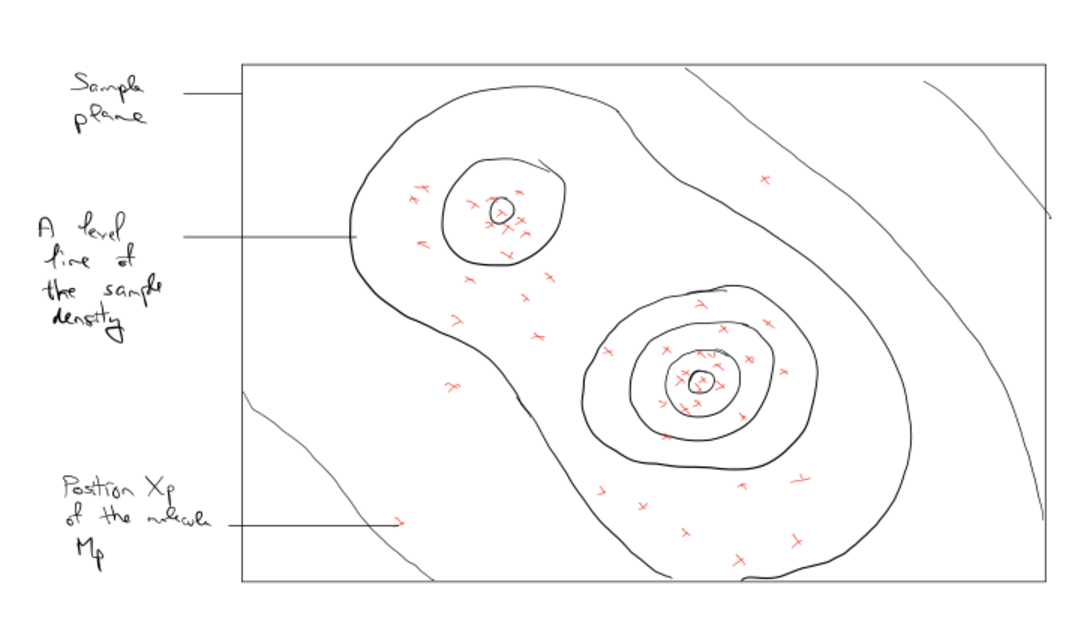
\includegraphics[scale = .5, keepaspectratio]{modelling/general/sample_distribution.pdf}
	\end{figure}
\end{frame}

\begin{frame}{General framework}{The sampling design}
\begin{itemize}
\item \underline{Discrete sampling:} the laser stops at $q$ different spots $(y_{1}, \hdots, y_{q})$ for a fixed duration $t_{0}$;
\item \underline{Continuous sampling:} the laser is driven along a path $\Gamma$ and its position at time $t$ is $\Gamma(t)$;
\end{itemize}

\begin{columns}[c]
	\begin{column}{5.75cm}
			\begin{figure}[H]
		\label{mapping1}\caption{Sampling design $(y_{1}, \hdots, y_{q})$ in spot mode}
		\centering
    	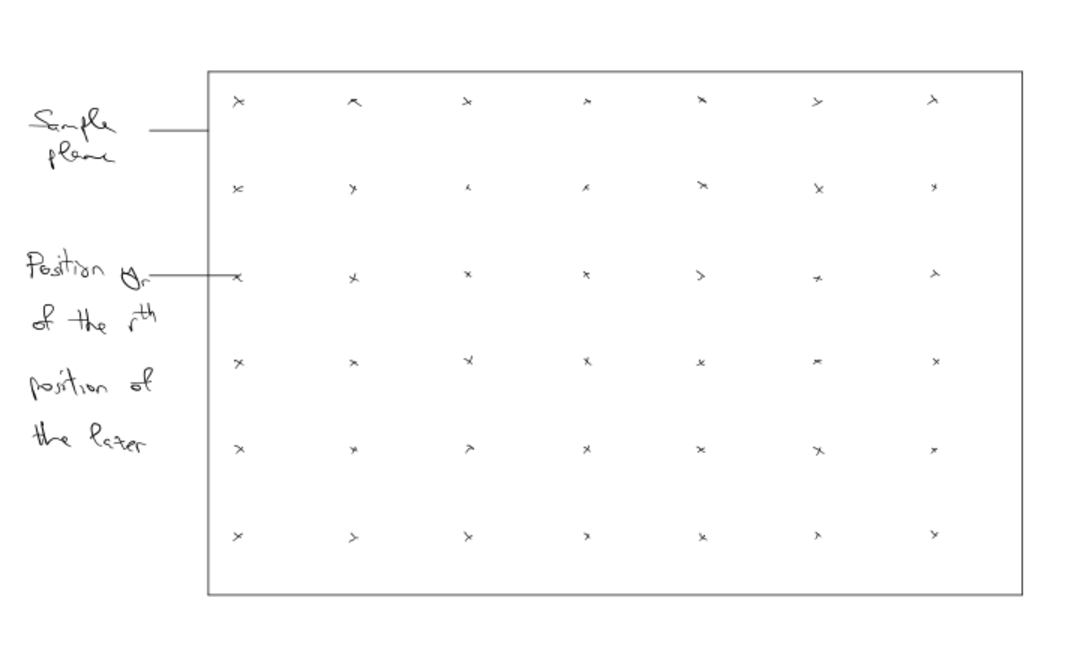
\includegraphics[width=\textwidth,height=\textheight,keepaspectratio]{modelling/general/sampling_design1.pdf}
	\end{figure}
	\end{column}
	\begin{column}{5.75cm}
			\begin{figure}[H]
		\label{mapping1}\caption{Sampling design $\Gamma$ in raster mode}
		\centering
    	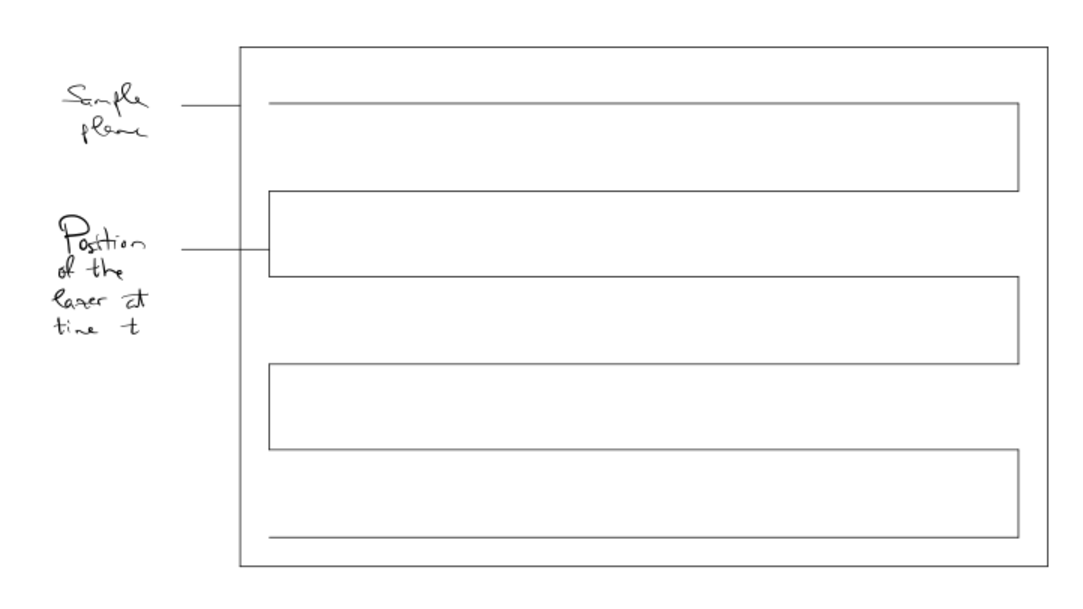
\includegraphics[width=\textwidth,height=\textheight,keepaspectratio]{modelling/general/sampling_design2.pdf}
	\end{figure}
	\end{column}
\end{columns}
\end{frame}

\begin{frame}{General framework}{The ionisation phenomenon I}
\begin{columns}[c]
	\begin{column}{5.75cm}
			\begin{figure}[H]
		\label{mapping1}\caption{Laser irradiance $I(x)$ in $W.m^{-2}$}
		\centering
    	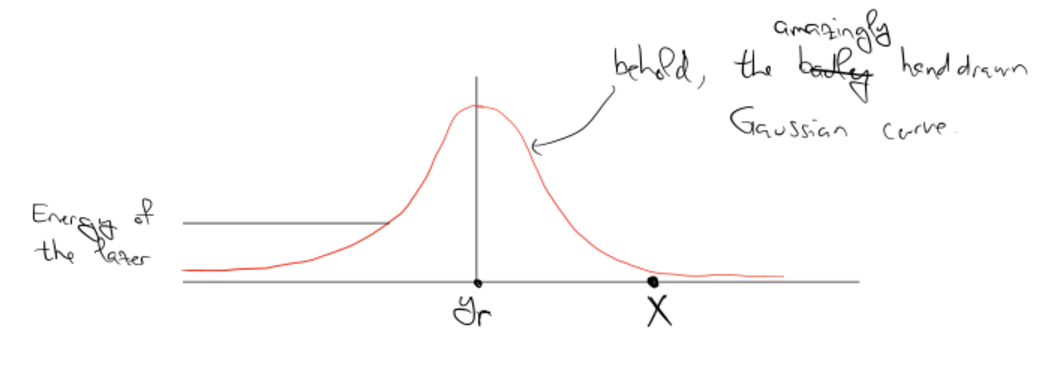
\includegraphics[width=\textwidth,height=\textheight,keepaspectratio]{modelling/general/ionisation1.pdf}
	\end{figure}
	\end{column}
	\begin{column}{5.75cm}
			\begin{figure}[H]
		\label{mapping1}\caption{Ionisation probability function $\mathcal{I}_{\mathds{P}}(t, y_{r} - X)$}
		\centering
    	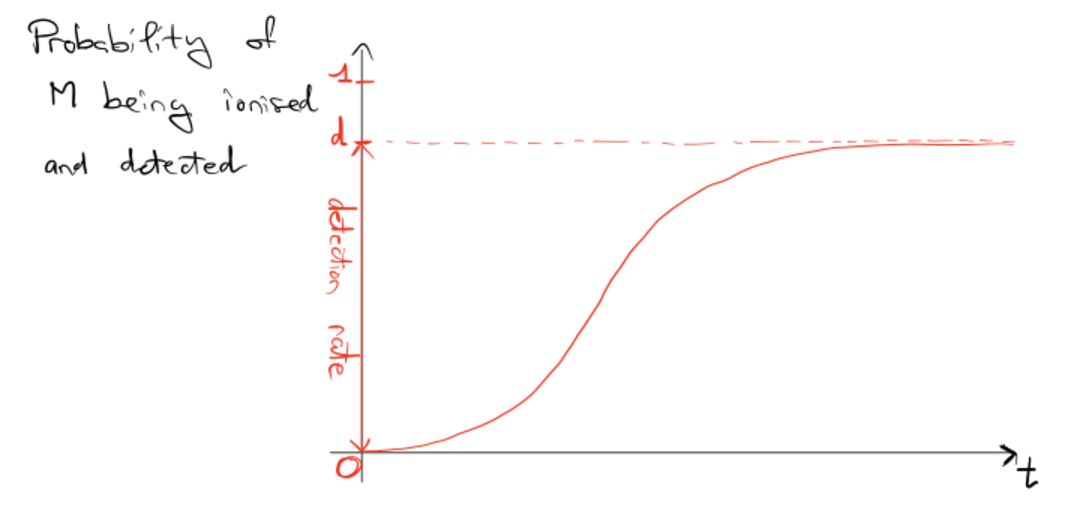
\includegraphics[width=\textwidth,height=\textheight,keepaspectratio]{modelling/general/ionisation2.pdf}
	\end{figure}
	\end{column}
\end{columns}
\end{frame}

\begin{frame}{General framework}{The ionisation phenomenon II}
\begin{figure}[H]
	\label{mapping1}\caption{Ionisation probability function $\mathcal{I}_{\mathds{P}}(t_{0}, y - x)$ for different values of $t_{0}$}
	\centering
    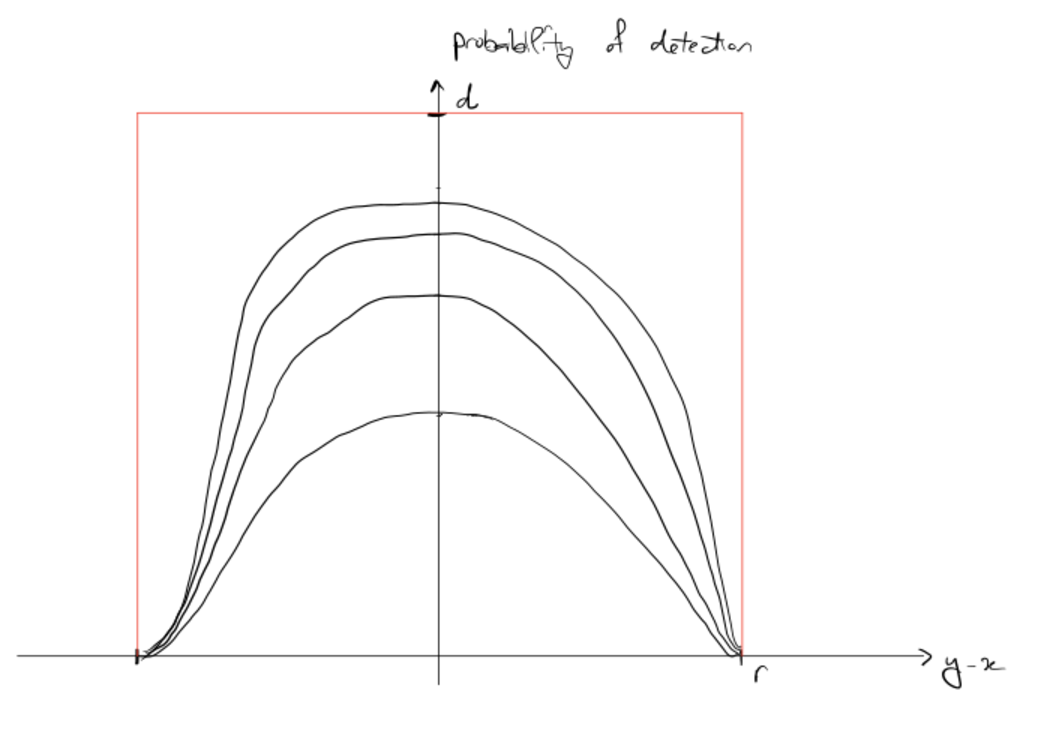
\includegraphics[scale = .45, keepaspectratio]{modelling/general/ionisation3.pdf}
\end{figure}
\end{frame}

\subsection{The (under)sampling case}
%%% MetaPost direct problem inference
\begin{frame}{Oversampling: where will we see the molecule?}
\underline{Recorded position:} $Y$ is the position of the laser when the molecule is detected;

\[\mathds{P}(Y = y_{r}) = (\mathcal{I}_{\mathds{P}}(t_{0}, \cdot) \star f_{x})(y_{r}) \cdot \prod\limits_{s = 1}^{r - 1} \left(1 - \left(\mathcal{I}_{\mathds{P}}(t_{0}, \cdot) \star f_{X}\right)(y_{s})\right)\]

\begin{figure}[H]
	\label{mapping1}\caption{The sampling design}
	\centering
    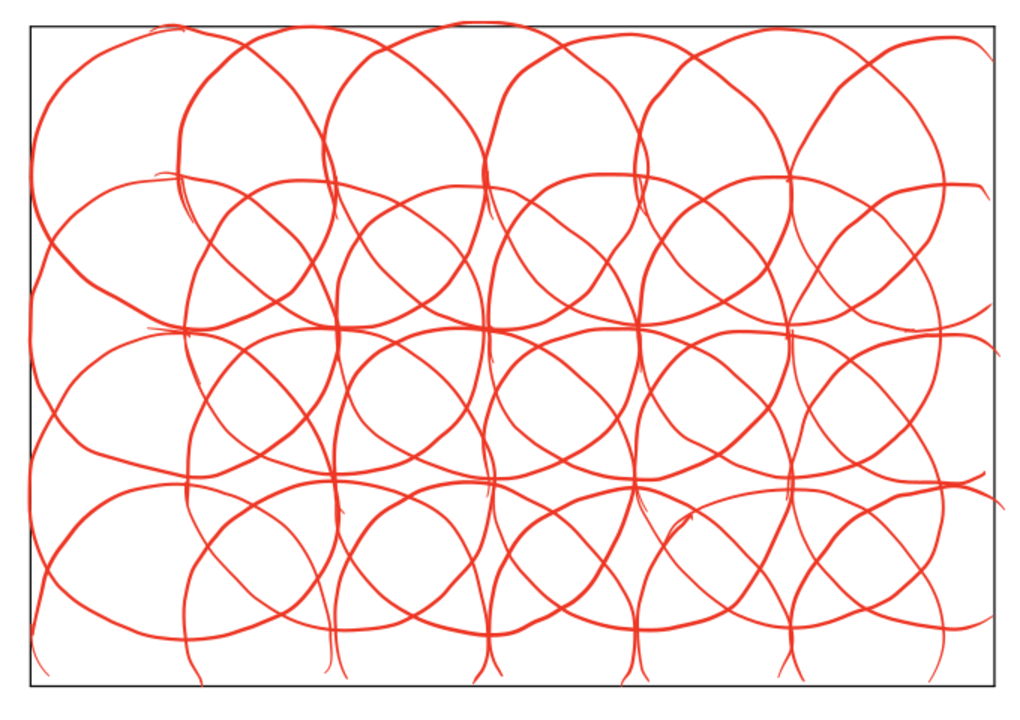
\includegraphics[scale = .3, keepaspectratio]{modelling/oversampling/oversampling.pdf}
\end{figure}

\end{frame}

%% MetaPost Inverse Problem inference
\begin{frame}{The (under)sampling case}{Distribution of the observation}
\underline{Image:}
\begin{itemize}
\item $1$ pixel = $1$ laser position
\item pixel $r$ contains $Z_{r} = \frac{1}{n} \sum\limits_{p = 1}^{n} \mathds{1}_{\{Y_{p} = y_{r}\}}$
\end{itemize}
\[\mathds{P}(Z_{r} = p) = {{n}\choose{n \cdot p}} \cdot \left((\mathcal{I}_{\mathds{P}}(t_{0}, \cdot) \star f_{X})(y_{r})\right)^{n \cdot p} \cdot \left(1 - (\mathcal{I}_{\mathds{P}}(t_{0}, \cdot) \star f_{X})(y_{r})\right)^{n \cdot (1 - p)}\]

\[ \mathds{E}\left[Z_{r}\right] = (\mathcal{I}_{\mathds{P}}(t_{0}, \cdot) \star f_{X})(y_{r}) \]

\[ \mathds{V}\left[Z_{r}\right] \leq \frac{1}{4 \cdot n} \]
\end{frame}

\subsection{The oversampling case}
%%% MetaPost direct problem inference
\begin{frame}{Oversampling: where will we see the molecule?}
\underline{Recorded position:} $Y$ is the position of the laser when the molecule is detected;

\[\mathds{P}(Y = y_{r}) = (\mathcal{I}_{\mathds{P}}(t_{0}, \cdot) \star f_{x})(y_{r}) \cdot \prod\limits_{s = 1}^{r - 1} \left(1 - \left(\mathcal{I}_{\mathds{P}}(t_{0}, \cdot) \star f_{X}\right)(y_{s})\right)\]

\begin{figure}[H]
	\label{mapping1}\caption{The sampling design}
	\centering
    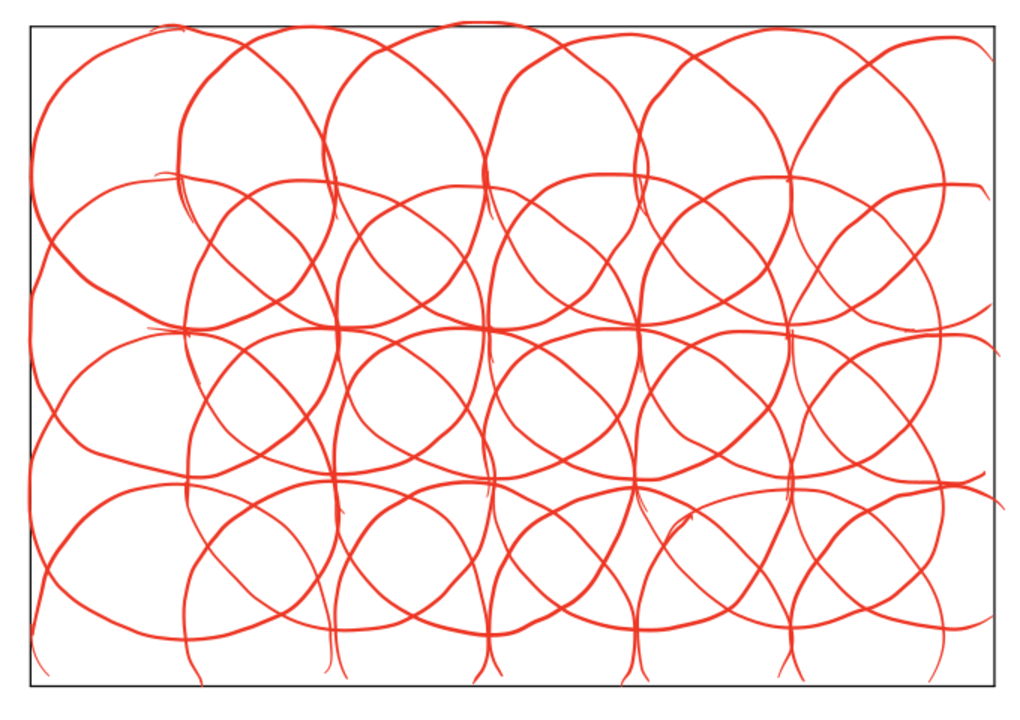
\includegraphics[scale = .3, keepaspectratio]{modelling/oversampling/oversampling.pdf}
\end{figure}

\end{frame}

%% MetaPost Inverse Problem inference
\begin{frame}{The (under)sampling case}{Distribution of the observation}
\underline{Image:}
\begin{itemize}
\item $1$ pixel = $1$ laser position
\item pixel $r$ contains $Z_{r} = \frac{1}{n} \sum\limits_{p = 1}^{n} \mathds{1}_{\{Y_{p} = y_{r}\}}$
\end{itemize}
\[\mathds{P}(Z_{r} = p) = {{n}\choose{n \cdot p}} \cdot \left((\mathcal{I}_{\mathds{P}}(t_{0}, \cdot) \star f_{X})(y_{r})\right)^{n \cdot p} \cdot \left(1 - (\mathcal{I}_{\mathds{P}}(t_{0}, \cdot) \star f_{X})(y_{r})\right)^{n \cdot (1 - p)}\]

\[ \mathds{E}\left[Z_{r}\right] = (\mathcal{I}_{\mathds{P}}(t_{0}, \cdot) \star f_{X})(y_{r}) \]

\[ \mathds{V}\left[Z_{r}\right] \leq \frac{1}{4 \cdot n} \]
\end{frame}
%
%\subsection{Raster mode}
%%%% MetaPost direct problem inference
\begin{frame}{Oversampling: where will we see the molecule?}
\underline{Recorded position:} $Y$ is the position of the laser when the molecule is detected;

\[\mathds{P}(Y = y_{r}) = (\mathcal{I}_{\mathds{P}}(t_{0}, \cdot) \star f_{x})(y_{r}) \cdot \prod\limits_{s = 1}^{r - 1} \left(1 - \left(\mathcal{I}_{\mathds{P}}(t_{0}, \cdot) \star f_{X}\right)(y_{s})\right)\]

\begin{figure}[H]
	\label{mapping1}\caption{The sampling design}
	\centering
    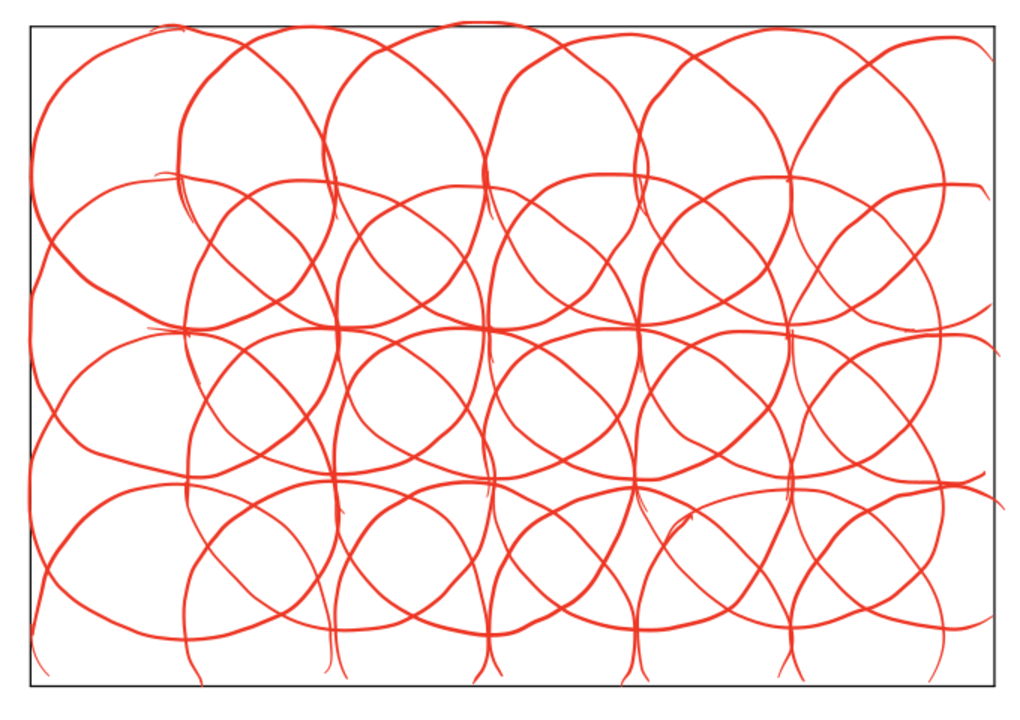
\includegraphics[scale = .3, keepaspectratio]{modelling/oversampling/oversampling.pdf}
\end{figure}

\end{frame}

%% MetaPost Inverse Problem inference
\begin{frame}{The (under)sampling case}{Distribution of the observation}
\underline{Image:}
\begin{itemize}
\item $1$ pixel = $1$ laser position
\item pixel $r$ contains $Z_{r} = \frac{1}{n} \sum\limits_{p = 1}^{n} \mathds{1}_{\{Y_{p} = y_{r}\}}$
\end{itemize}
\[\mathds{P}(Z_{r} = p) = {{n}\choose{n \cdot p}} \cdot \left((\mathcal{I}_{\mathds{P}}(t_{0}, \cdot) \star f_{X})(y_{r})\right)^{n \cdot p} \cdot \left(1 - (\mathcal{I}_{\mathds{P}}(t_{0}, \cdot) \star f_{X})(y_{r})\right)^{n \cdot (1 - p)}\]

\[ \mathds{E}\left[Z_{r}\right] = (\mathcal{I}_{\mathds{P}}(t_{0}, \cdot) \star f_{X})(y_{r}) \]

\[ \mathds{V}\left[Z_{r}\right] \leq \frac{1}{4 \cdot n} \]
\end{frame}
